\documentclass[cs4size,a4paper,adobefonts]{ctexart}
\usepackage{amsmath,amsthm,amssymb}
\usepackage[colorlinks=true,allcolors=black]{hyperref}
\usepackage{indentfirst}
\usepackage[a4paper,left=2.5cm,right=2.5cm,bottom=2.5cm,top=2.5cm]{geometry}
\usepackage{graphicx}
\usepackage{subcaption}
\usepackage{url}
\usepackage{fontspec}
\setmainfont{Palatino}
\setmonofont[Scale=MatchLowercase]{Monaco}
\pagestyle{plain}
\punctstyle{kaiming}
\usepackage{unicode-math}
\setmathfont{Asana Math}

\newcommand{\GridMaze}{\href{http://itunes.apple.com/app/grid-maze/id553265800?mt=8}{Grid Maze}}
\graphicspath{{pic/}}

\begin{document}
\title{{\bfseries 算法有什么用}\\\large 略述 \GridMaze{} 里的算法}
\author{\href{mailto:txyyss@gmail.com}{王盛颐}}
\date{}
\maketitle

\section*{缘起}
最近我的 iPad 程序 \GridMaze{} 在历经了 5 个月的开发,13 天的审核之后,
终于在苹果应用商店上架了。这个程序的主要功能是能根据输入的文字或图案,
生成一个迷宫,使得走出这个迷宫的唯一路径能形成当初输入的文字或图案。

生成这样一个迷宫的想法最早可以追溯到 2007 年底,不过那时完全不知道该怎
么做,于是这个想法也就是在脑子里徘徊了一阵,就置之一旁了。直到一年后也
就是 2008 年底,在看到一篇根据图形生成迷宫轮廓的文章
\cite{Xu:2007:ImageMaze}时,我突然想明白该怎么做了,于是就用
Mathematica 做了一些试验验证了我的想法,之后就一边完善想法一边写程序,
直到做出了一个以我名字为解法的迷宫。这个原型程序也就因为目标已达成而被
束之高阁。2010年,在朋友的鼓励下,我用 Qt 写了这个迷宫生成程序的界面,
同时用 C++ 重写了原先用 Java 和 Mathematica 写的部分,完善了一些功能,
这就是
\href{https://sites.google.com/site/txyyss/projects/text-maze-creator}{Text
  Maze Creator}。这个程序依赖一个第三方的 TSP 求解程序和一个
ActionScript 的编译器,操作起来很复杂,所以也没有提供下载,只是放了一些
样例在网上。转眼就到了2012 年,由于陆续能收到请求生成迷宫的邮件,我决定
写一个大家都能用的迷宫生成程序。我重新设计了界面,自己写了 TSP 的求解算
法,这才有了 iPad 上的 \GridMaze。

在开发 \GridMaze{} 的过程中,我遇到了很多有意思的问题,为了解决这些问题
参考和设计了很多算法。我觉得有必要把这些问题和解决办法整理一番,也算是
在初步完成这个项目之后,做一个总结报告。

\section{概述}
名不正则言不顺,言不顺则事不成。我先明确一下要解决的问题:生成一个迷宫,
使得走出这个迷宫的唯一路径能形成指定的文字或图案。这句话不够精确,需要
进一步的解释来消除歧义。

首先是“迷宫”的意思。本文的迷宫专指一种需要玩家从一个指定的起点出发,在
用墙隔断形成的分叉道路中辨识选择,最终到达指定终点的游戏。这样的迷宫具
有很多种形式(图 \ref{fig:manyMazes}),我要生成的迷宫是外轮廓为矩形,
分叉道路横平竖直,每一段墙的长度为单位长度整数倍的,解法唯一的所谓“标准
迷宫”(图 \ref{fig:rectMaze})。

\begin{figure}[htbp]
  \centering
  \begin{subfigure}[c]{0.31\textwidth}
    \centering
    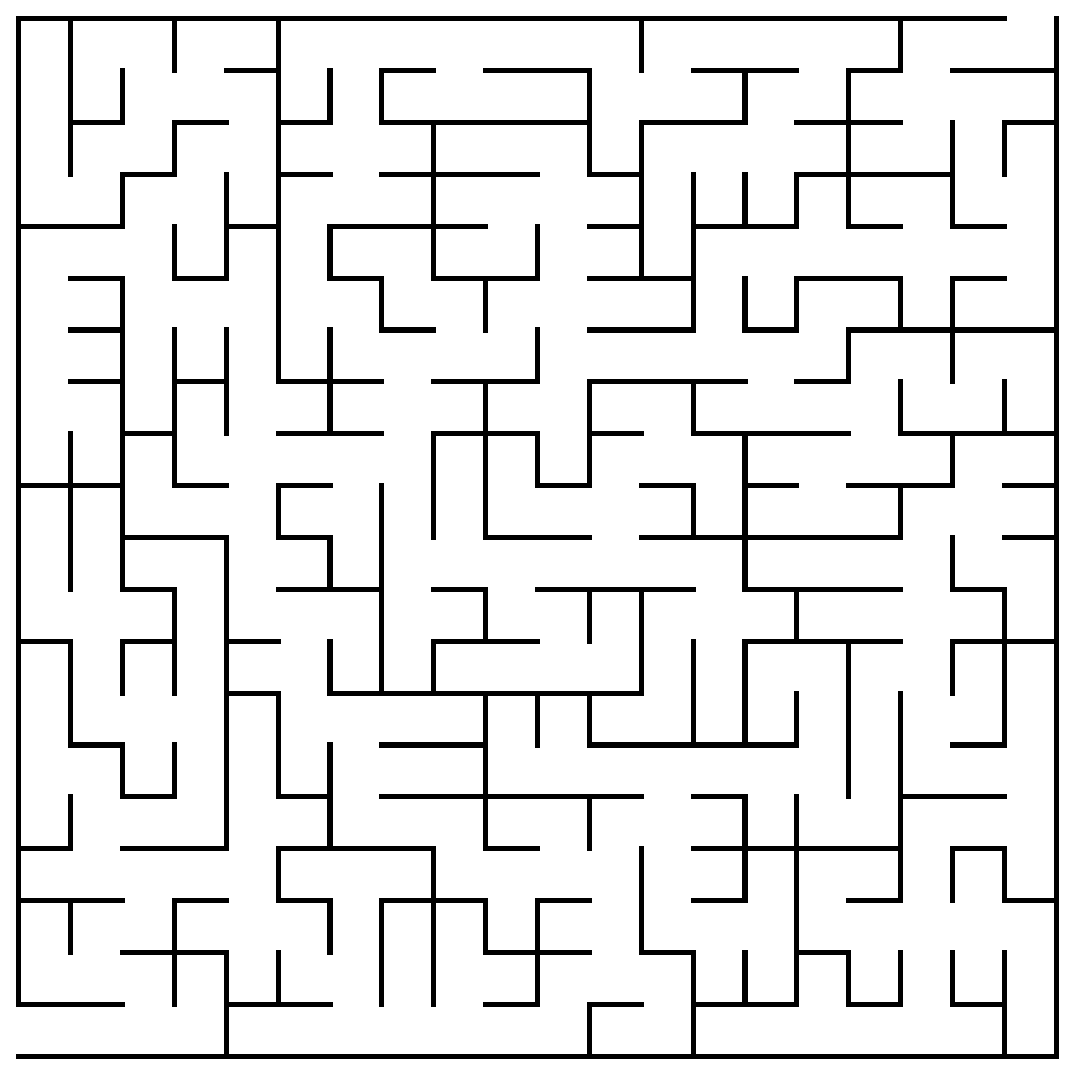
\includegraphics[width=\textwidth]{rectMaze}
    \caption{标准迷宫}\label{fig:rectMaze}
  \end{subfigure}
  ~
  \begin{subfigure}[c]{0.31\textwidth}
    \centering
    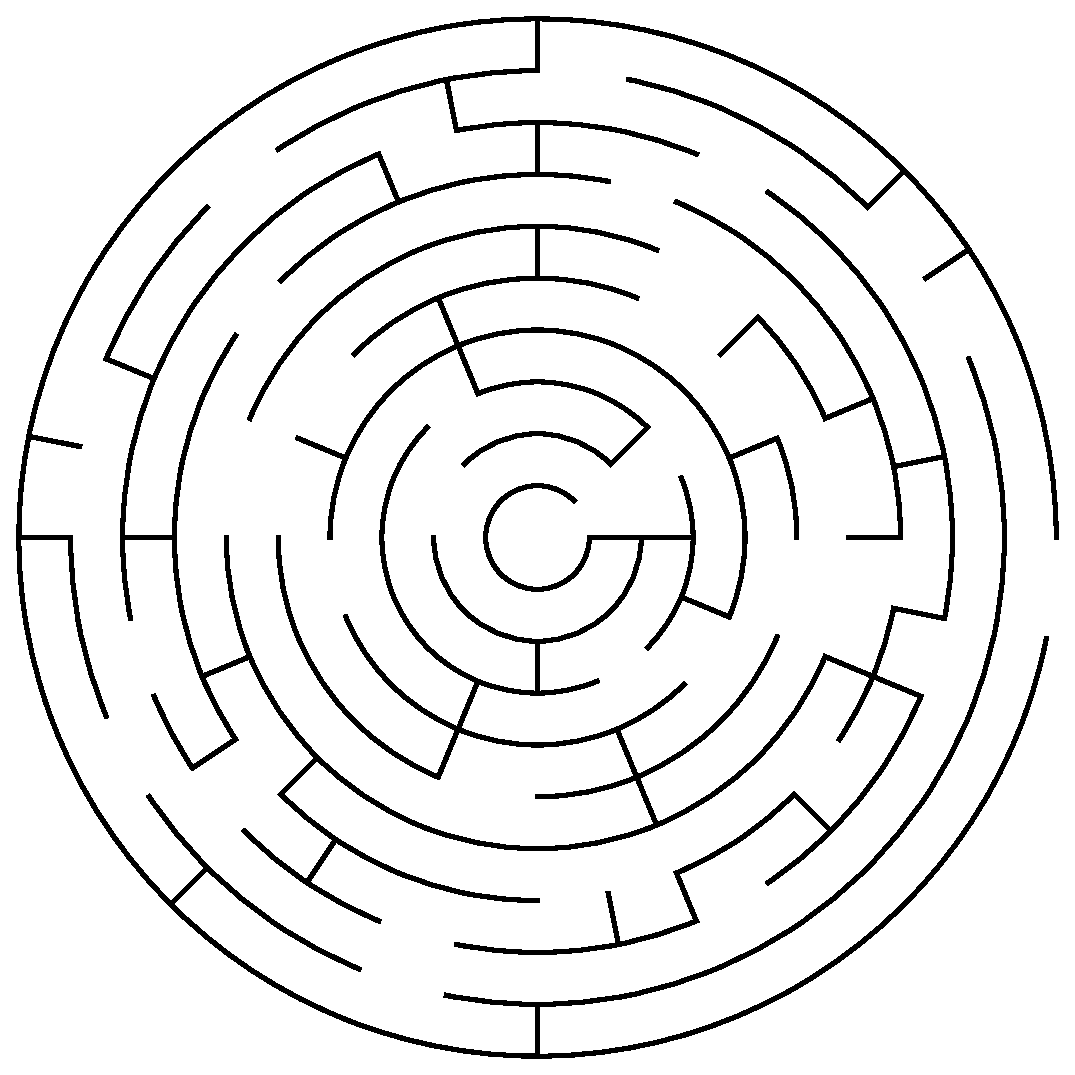
\includegraphics[width=\textwidth]{diskMaze}
    \caption{圆形迷宫}\label{fig:diskMaze}
  \end{subfigure}
  ~
  \begin{subfigure}[c]{0.31\textwidth}
    \centering
    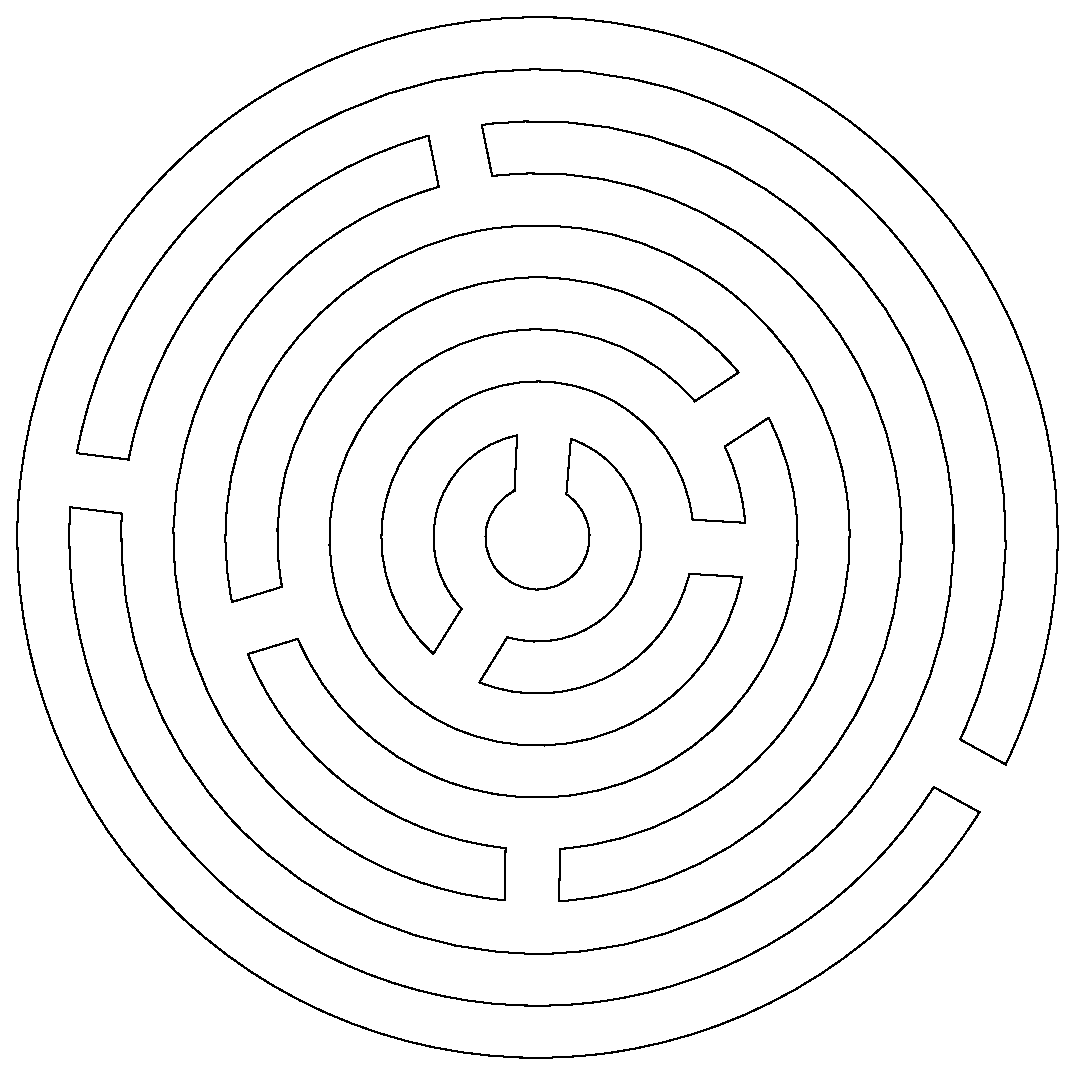
\includegraphics[width=\textwidth]{eulerMaze}
    \caption{一笔画迷宫}
  \end{subfigure}
  \caption{各种不同类型的迷宫}\label{fig:manyMazes}
\end{figure}

接下来定义什么叫“路径形成指定的文字或图案”。我将文字或图案变成点阵(如
  图 \ref{fig:abcGrid}),如果有条路径能把这个点阵串起来,并且这条路径
上只遗漏了少量点阵中的点,只增加了少量不在这个点阵中的点。那么就可以说
路径形成了指定的文字或图案(如图 \ref{fig:abcPath})。当然,由于这条路
径还要是“标准迷宫”的解答路径,所以还必须加上横平竖直,自身无交叉两个额
外的条件。

\begin{figure}[htbp]
  \centering
  \begin{minipage}{0.5\textwidth}
    \centering
    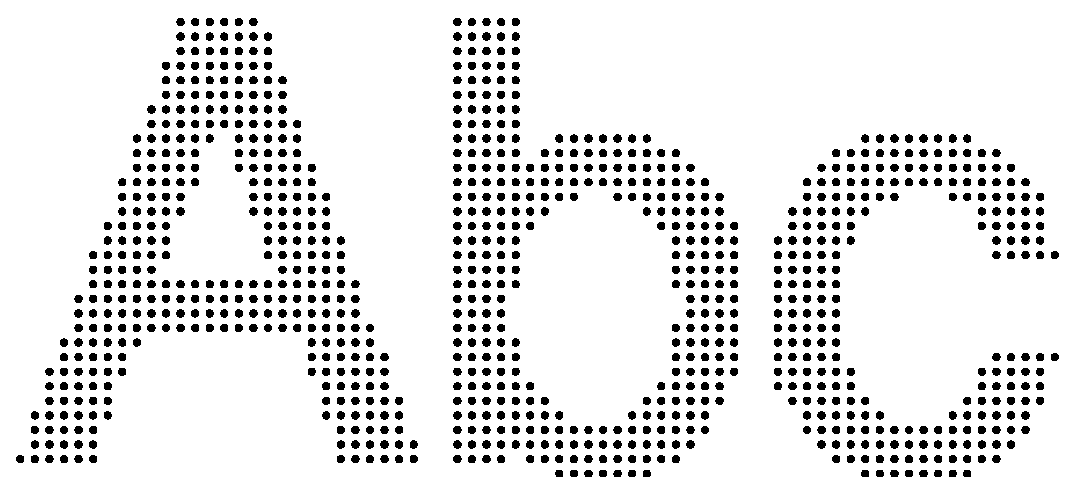
\includegraphics[width=0.95\linewidth]{abcGrid}
    \caption{文字点阵}\label{fig:abcGrid}
  \end{minipage}%
  \begin{minipage}{0.5\textwidth}
    \centering
    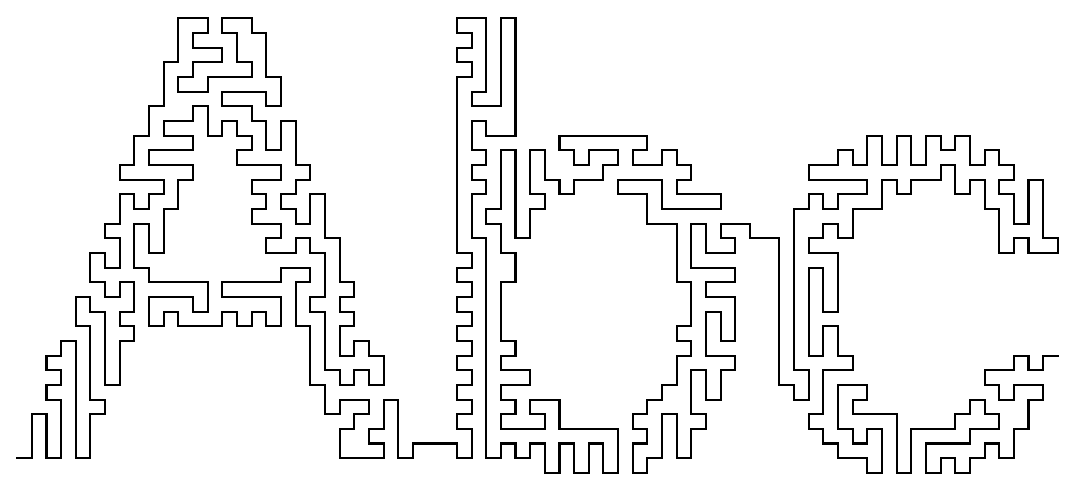
\includegraphics[width=0.95\linewidth]{abcPath}
    \caption{路径形成的文字}\label{fig:abcPath}
  \end{minipage}
\end{figure}

在明确了这两点之后,要解决的问题就清楚了。首先要根据点阵生成解答路径,
其次要根据解答路径生成迷宫。通过进一步的思考我发现,生成路径这个问题比
生成迷宫要困难得多。本着先易后难的原则,下面我先介绍如何根据已有的解答
路径,生成迷宫。

\section{迷宫生成算法}
生成迷宫有许多种算法 \cite{wiki:mazeGen}。我用的是基于图论的生成方法。
从一组预先安排好的互相隔断的格子布局开始,从这布局可以定义一个无向图
$G=(V,E)$,结点集合 $V$ 就是全部的格子,边的集合 $E$ 定义如下:若格子
$a,b$ 位于一堵墙的两侧,则 $\{a,b\}\in E$。

对任意 $F\subset E$,图 $G$ 的子图 $S=(V,F)$ 都对应一个迷宫,反之亦然。
具体对应方法如下:在原来布局的基础上,若 $e\in F$,则拆掉边 $e$ 对应的
那堵墙,也就是说 $S$ 的边意味着迷宫的通路。若 $S$ 不连通,那意味着对应
的迷宫有格子不可达,这显然不够理想。若 $S$ 中出现环路,则意味着迷宫的求
解路径可能不止一条,这也不理想。所以一个理想的迷宫对应的子图 $S$ 全连通
且无环,这正是图 $G$ 的支撑树 (Spanning Tree)。

\begin{figure}[htbp]
  \centering
  \begin{subfigure}[c]{0.31\textwidth}
    \centering
    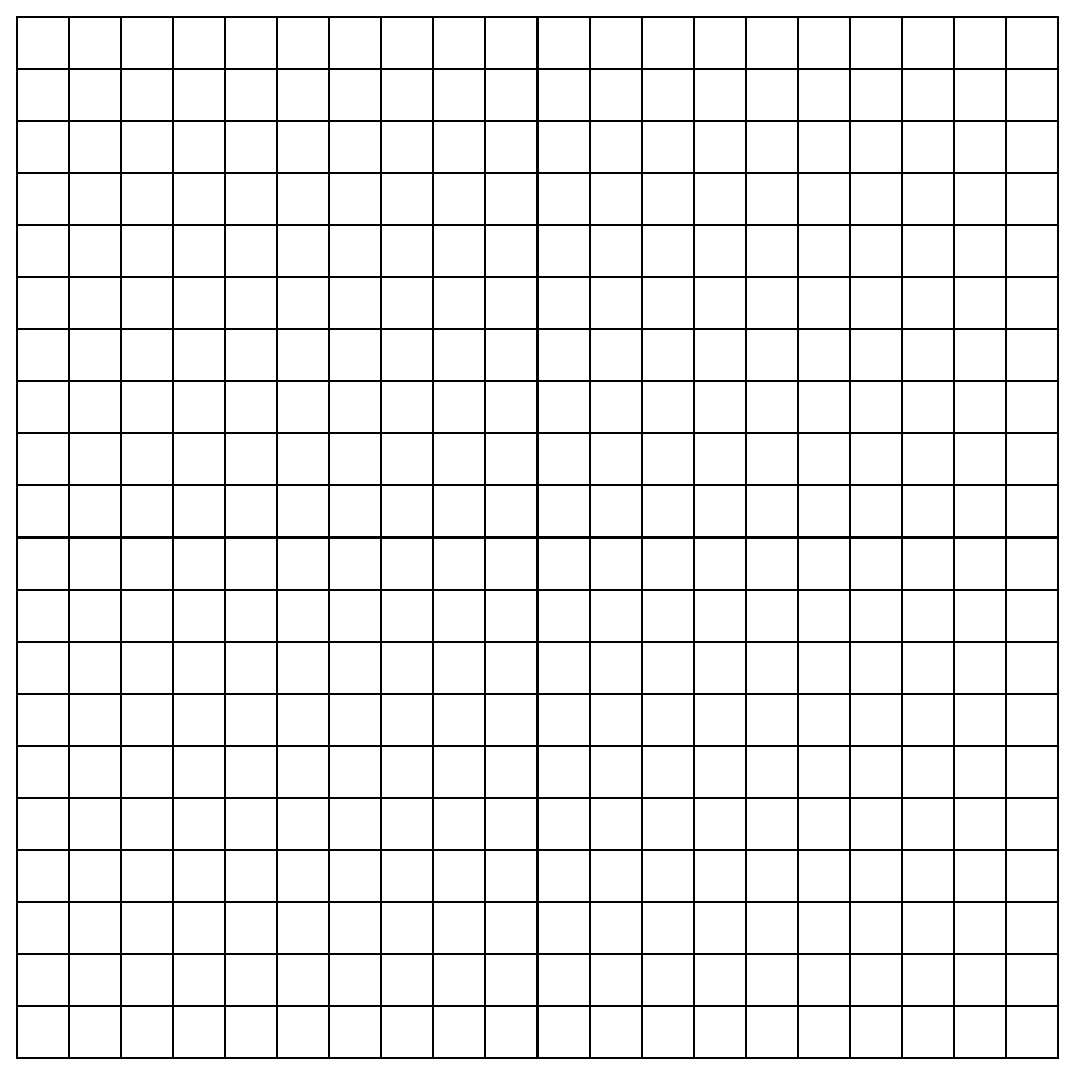
\includegraphics[width=\textwidth]{rectCells}
    \caption{标准迷宫的格子布局}
  \end{subfigure}
  ~
  \begin{subfigure}[c]{0.31\textwidth}
    \centering
    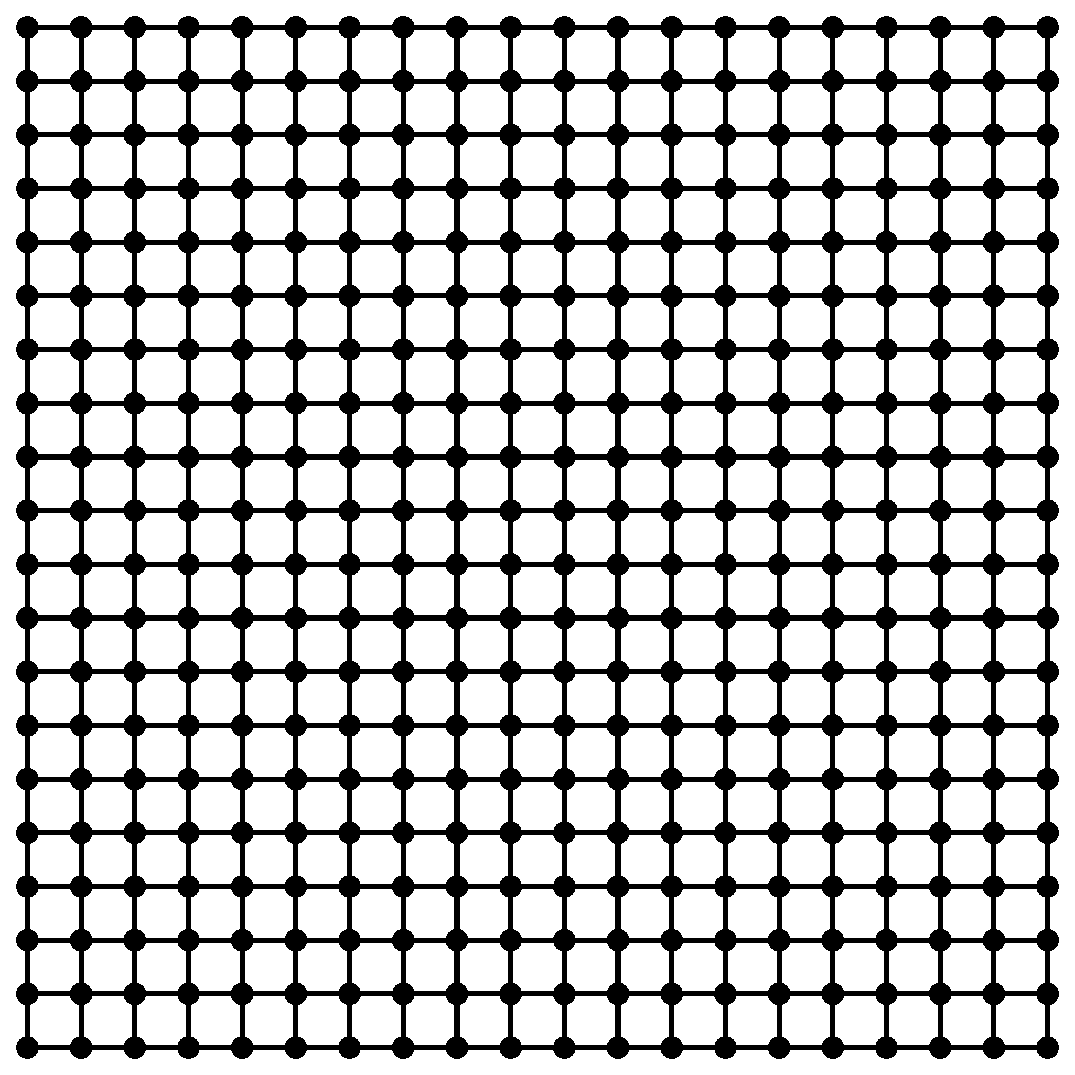
\includegraphics[width=\textwidth]{rectGraph}
    \caption{布局对应的无向图 $G$}
  \end{subfigure}
  ~
  \begin{subfigure}[c]{0.31\textwidth}
    \centering
    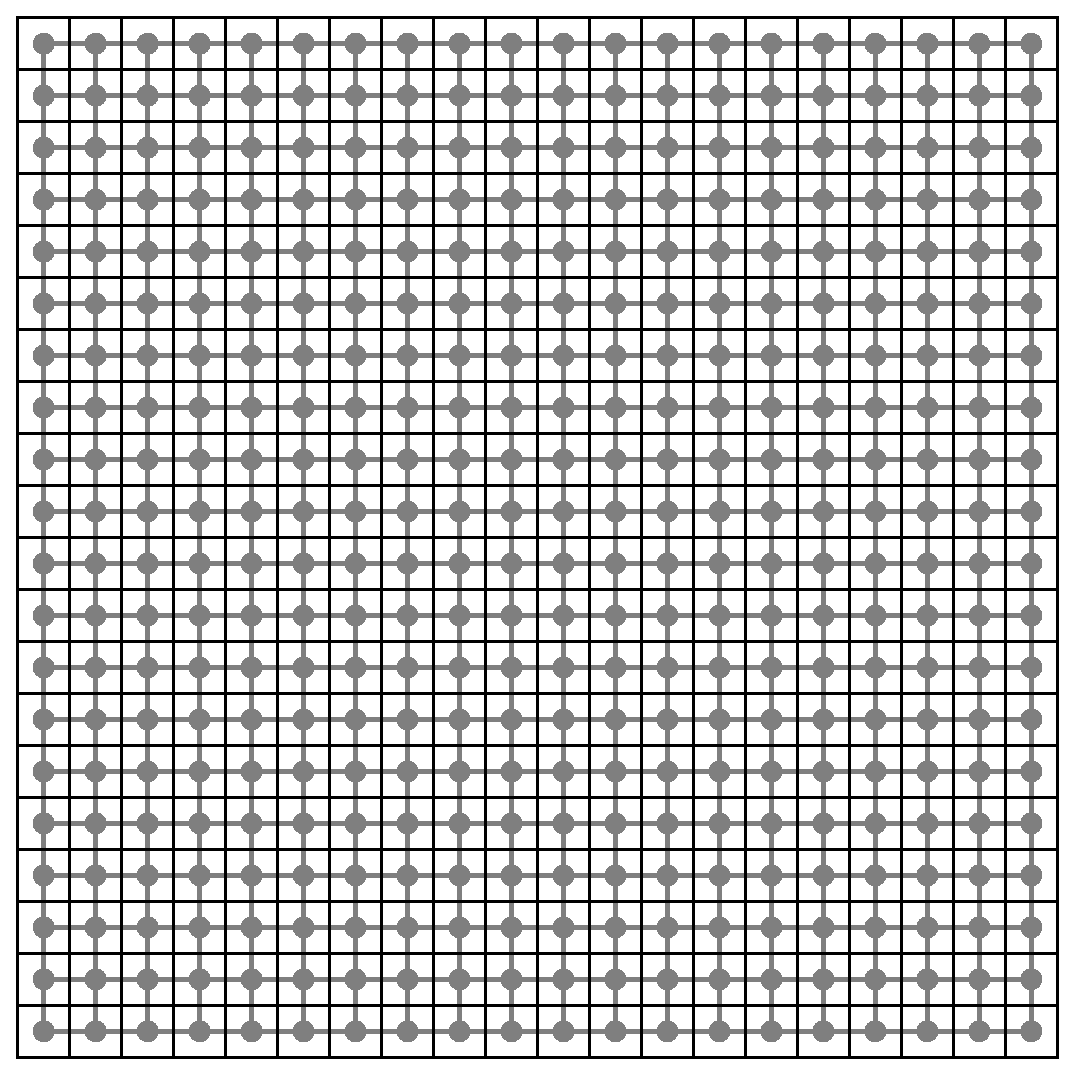
\includegraphics[width=\textwidth]{rectMerged}
    \caption{将布局和图合并在一起}
  \end{subfigure}
  \caption{标准迷宫的布局和由它定义的无向图}\label{fig:rectMazeGen}
\end{figure}

到这里一个普通迷宫的生成算法就很显然了,任意计算支撑树的算法都可以。比
如随机 Kruskal 算法:
\begin{enumerate}
\item 创建一个全部墙的列表 $l$,给每个格子创建一个集合,该集合开始只包
  含那个格子一个元素
\item 乱序遍历 $l$,遍历时做如下操作:
  \begin{itemize}
  \item 若墙两边的格子属于一个集合,则不做任何操作
  \item 若强两边的格子不在一个集合里,则拆除这堵墙,合并两边格子所在的集合
  \end{itemize}
\end{enumerate}

\begin{figure}[htbp]
  \centering
  \begin{subfigure}[c]{0.31\textwidth}
    \centering
    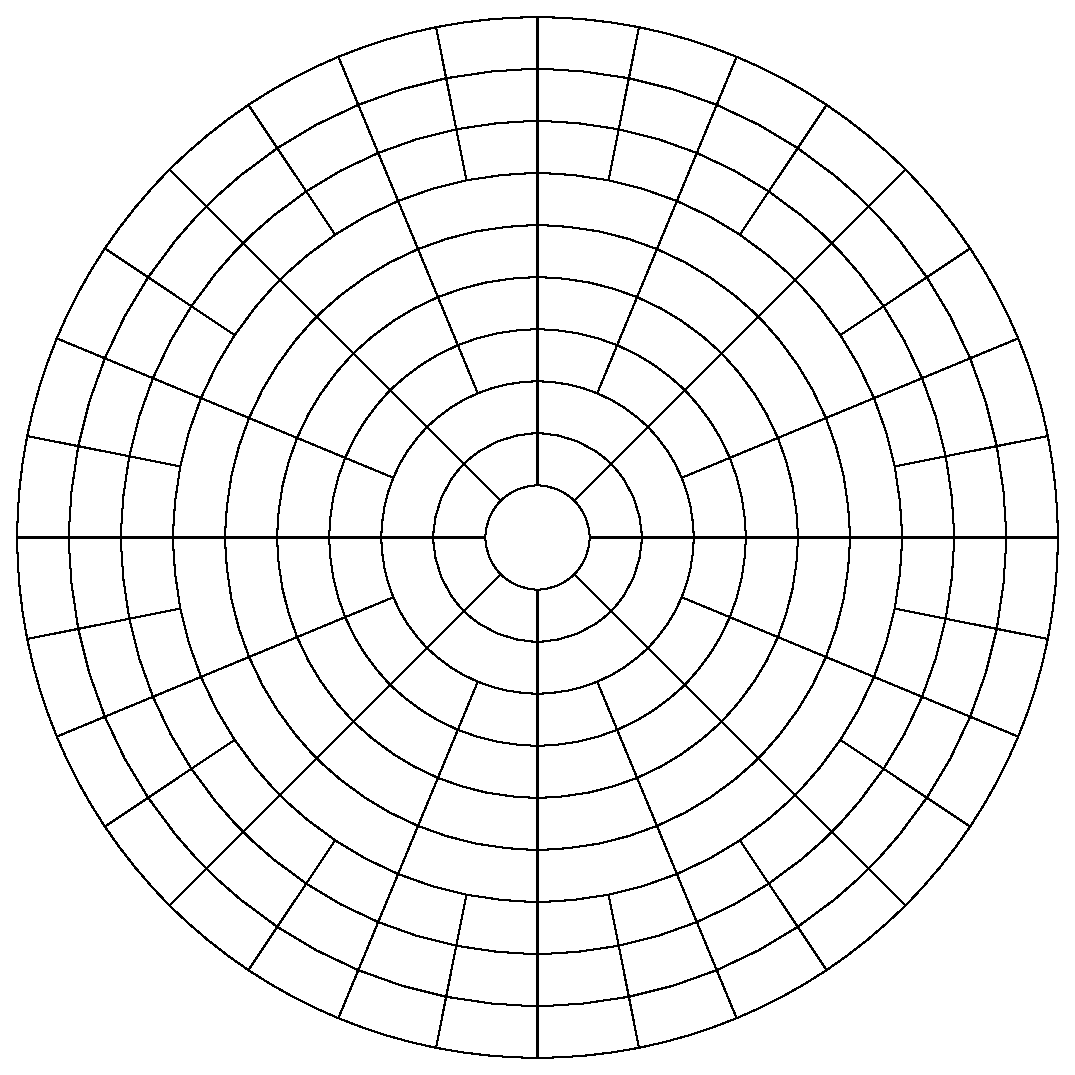
\includegraphics[width=\textwidth]{diskCells}
    \caption{圆形迷宫的格子布局}
  \end{subfigure}
  ~
  \begin{subfigure}[c]{0.31\textwidth}
    \centering
    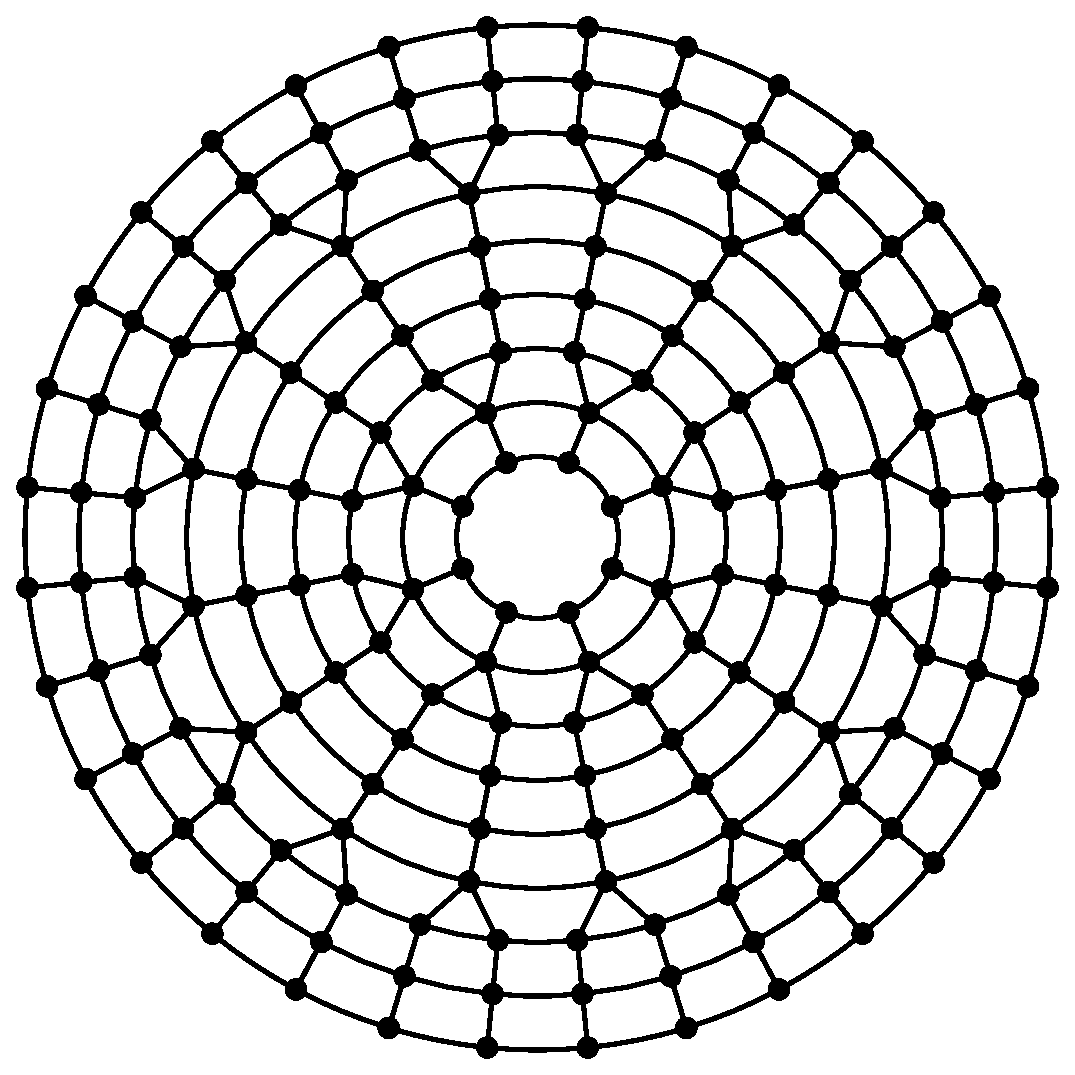
\includegraphics[width=\textwidth]{diskGraph}
    \caption{布局对应的无向图 $G$}
  \end{subfigure}
  ~
  \begin{subfigure}[c]{0.31\textwidth}
    \centering
    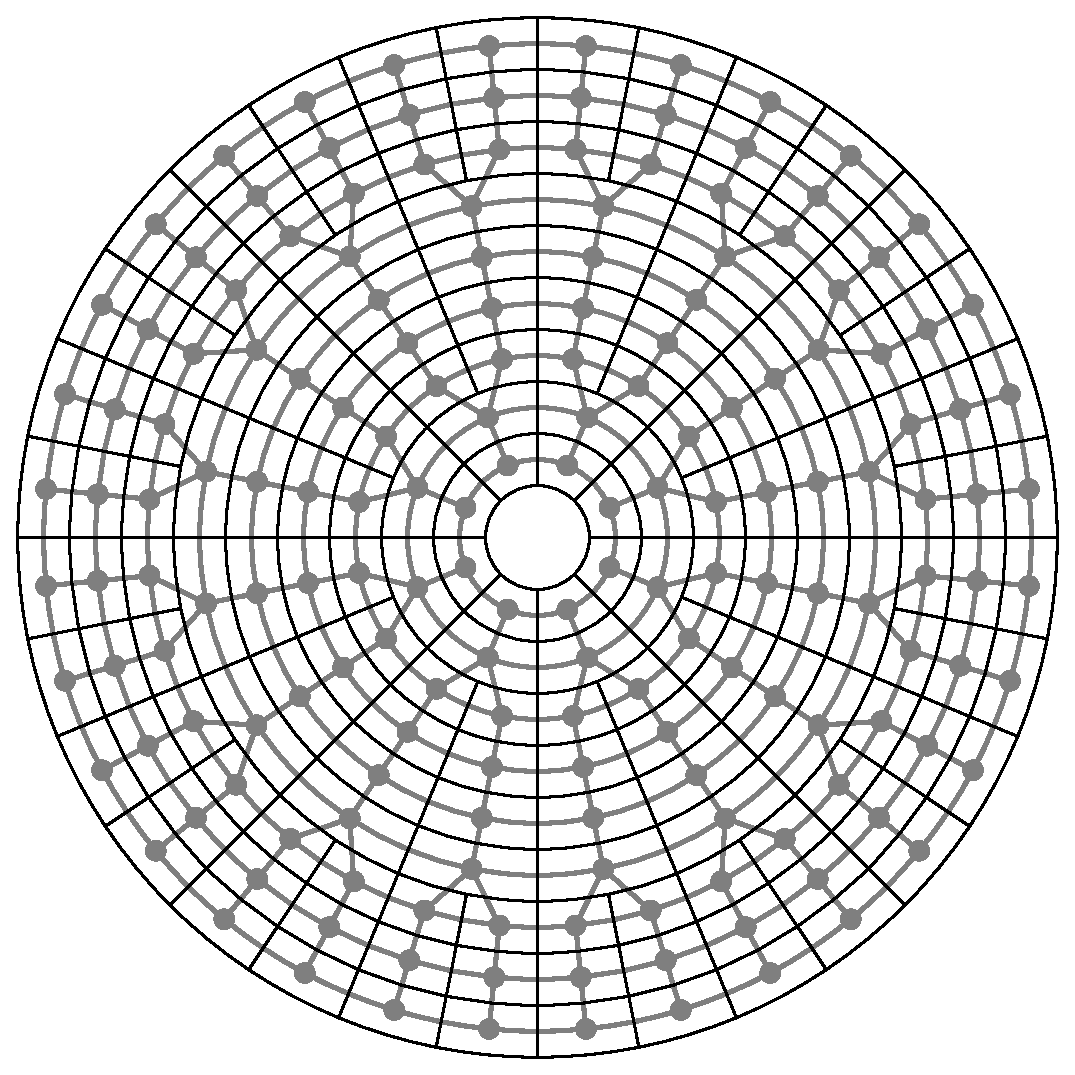
\includegraphics[width=\textwidth]{diskMerged}
    \caption{将布局和图合并在一起}
  \end{subfigure}
  \caption{圆形迷宫的布局和由它定义的无向图}\label{fig:diskMazeGen}
\end{figure}

图 \ref{fig:rectMaze} 中的标准迷宫和图 \ref{fig:diskMaze} 中的圆形迷宫
都是用随机 Kruskal 算法分别根据图 \ref{fig:rectMazeGen} 和图
\ref{fig:diskMazeGen} 中的布局生成的。有了这个算法,根据已有解答路径生
成迷宫变得轻而易举。只要把算法中 $l$ 的遍历顺序修改一下,先遍历解答路径
经过的那些墙,而后乱序遍历即可。

值得一提的是,随机 Kruskal 算法中,大量需要进行集合查找和集合合并的操作,
且这些集合彼此不相交。这可以用一种叫并查集 (Disjoint Sets) 的数据结构来
进行。这种数据结构单步进行查找或合并操作的时间复杂度几乎是常数,所以用
了这一数据结构的随机 Kruskal 算法的时间复杂度是 $O(n)$ 的,$n$ 是墙的数
量。关于 Disjoint Set 这里就不细说了,有兴趣的读者可查阅 \cite{clrs} 的
第 21 章。

\section{点阵连成路径的算法}
和生成迷宫相比,把点阵连成不自交的,横平竖直的路径要困难得多。下面将从
问题的进一步分析开始,逐步说明解决这一问题的方法。

\subsection{问题的进一步分析}

点阵的每个点都是坐标为整数的整点,如果把其中距离为 1 的点连起来,就形成
了一个格点图 (Grid Graph)。我们的问题就变成了能不能在这个格点图上找到指
定起始点的一条经过所有点而不自交的路径,也即所谓的哈密尔顿路径
(Hamiltonian path)。如果不能,那能不能通过添加或减少尽可能少的格点,使
之成为可能。非常遗憾,在一般的图上找哈密尔顿路径是 NP 完全的
\cite{Garey:1979:CIG:578533},这正是把点阵连成求解路径这一问题困难所在。

在一般的图上找哈密尔顿路径是 NP 完全问题,现在要解决的问题并不是一般的
图,是格点图啊。它有很多良好的性质,比如它是平面图,是二分图,每个点的
度数不超过 4。在它上面找哈密尔顿路径是不是要简单些呢?早在 1982 年就有
人想过这个问题,并给出了否定的答案 \cite{citeulike:1905588}。到了 1997
年 Lenhart 等人倒是给出了多项式时间的在没有洞的格点图上找到哈密尔顿回路
的算法 \cite{Lenhart:1997:HCS:795663.796334},但我的问题中的图不可避免
会有洞,所以这个结果还是对我没用。这里特别说明一下,一般的哈密尔顿路径
问题只要添加一个连接起始点的额外的点就能变成一个哈密尔顿回路问题,格点
图的话,无非添加若干格点也能同样转化。所以只要有哈密尔顿回路问题的解法
也就能解决哈密尔顿路径问题了。

理论上证明这是十分困难的 NP 完全问题了,那下面能想的就是近似解法。清华
大学 2011 年的文章 \cite{Zhang20115340} 给出了一类特殊的连通格点图上复
杂度为 $O(n^2)$ 的找哈密尔顿回路的近似解法,但还是不能解决一般格点图上
的问题。我还是只能采取 2008 年想到的办法:先求一个 TSP 近似解,然后局部
修正。

TSP(Travelling Salesman Problem) 是旅行推销员问题的意思,它是组合优化中
赫赫有名的一个 NP-hard 问题 \cite{wiki:TSP}。TSP 可以定义成在一个无向带
权图中找一条遍历所有结点的回路或路径,使得这条回路或路径上边的权重之和
最小。如果这个图的结点是平面上的点,图是所有点的完全图,而边的权重是边
连接的两个点之间的欧氏距离,这种特殊的 TSP 可称为欧几里德TSP
(Euclidean TSP),它纯由平面上的点决定,它和一般 TSP 差不多,是个 NP 完
全问题。如果格点图上存在哈密尔顿路径,那么这条路径也是由这些格点决定的
欧几里德 TSP 的解路径,因为不可能由比长度 $n-1$ 更短的连接 $n$ 个格点的
路径了。反之则未必,因为欧几里德 TSP 并不能保证解路径一定横平竖直(不自
  交是显然的)。若欧氏 TSP 的解不是横平竖直,那说明肯定不存在哈密尔顿路
径了,但通常可以通过局部修正这个解路径,也即增删点的方法,让这个解路径
横平竖直而成为我们要求的用于生成迷宫的解答路径。

有了上面的认识,算法就有了:近似求解欧几里德 TSP 问题,修正解路径。若修
正不成功,则对问题做微小扰动然后重复“求解、修正”的循环,直到找到横平竖
直的路径为止。从实践看,这个算法还是能结束的。下文如过不做特殊说明,所
提到的 TSP 均指欧几里德 TSP。

\subsection{TSP 的近似解法}
TSP 这个问题是如此有名,关于它的研究论文几十年来可谓汗牛充栋。2011 年出
版的 \cite{cook2011pursuit} 详述了这个问题的源流,对于它的解法更是叙述
的重中之重。但书中限于篇幅并没有说明白求解算法的技术细节。根据书中的线
索我找到了一篇技术报告 \cite{1999finding},这里面详细叙述了寻找 TSP 回
路的近似算法。\GridMaze{} 的算法主要便是依据这篇报告中的算法修改而来。
我之所以要修改,是因为报告中只有求 TSP 回路的算法,我要求的是起点和终点
不同的一条路径。我并没有把求路径的问题转换成求回路的问题,然后用原始算
法求解。我直接修改了求回路的算法,使之能用于求指定了起点和终点的遍历路
径。

\cite{1999finding} 中的算法又被称为 Lin-Kernighan 算法。它的基本想法很
简单:先找到一条初始的遍历路径,然后逐步迭代优化。

\subsubsection{寻找初始遍历路径}
Lin-Kernighan 算法对初始遍历路径并没有什么特别的要求,任意一条遍历所有
点的路径均可。但如果初始路径本身长度就比较短,那可以减少后续迭代优化的
时间和次数。若 TSP 问题的最优解长度为 $l$,那么通过以适当顺序遍历这平面
上 $n$ 个点的欧几里德最小生成树 (Euclidean Minimum Spanning Tree,
EMST),可得到长度不大于 $2l$ 的遍历路径,这比随便找一条随机路径好多了。

求一般图的最小生成树的 Kruskal 算法,其时间复杂度为 $O(E\log V)$,$E$
是边的数量,$V$ 是点的数量。若预先将边按长度安排好序,并采用并查集
(Disjoint Sets) 做为数据结构,时间复杂度可降为 $O(E\alpha(V))$。
$\alpha$ 是 Ackermann 函数的反函数,几乎可以认为是个常数。即便如此,对
EMST 问题来讲,由于图是完全图,直接使用 Kruskal 算法时间复杂度仍然有
$O(n^2)$ 这么高。 

\begin{figure}[htbp]
  \centering
  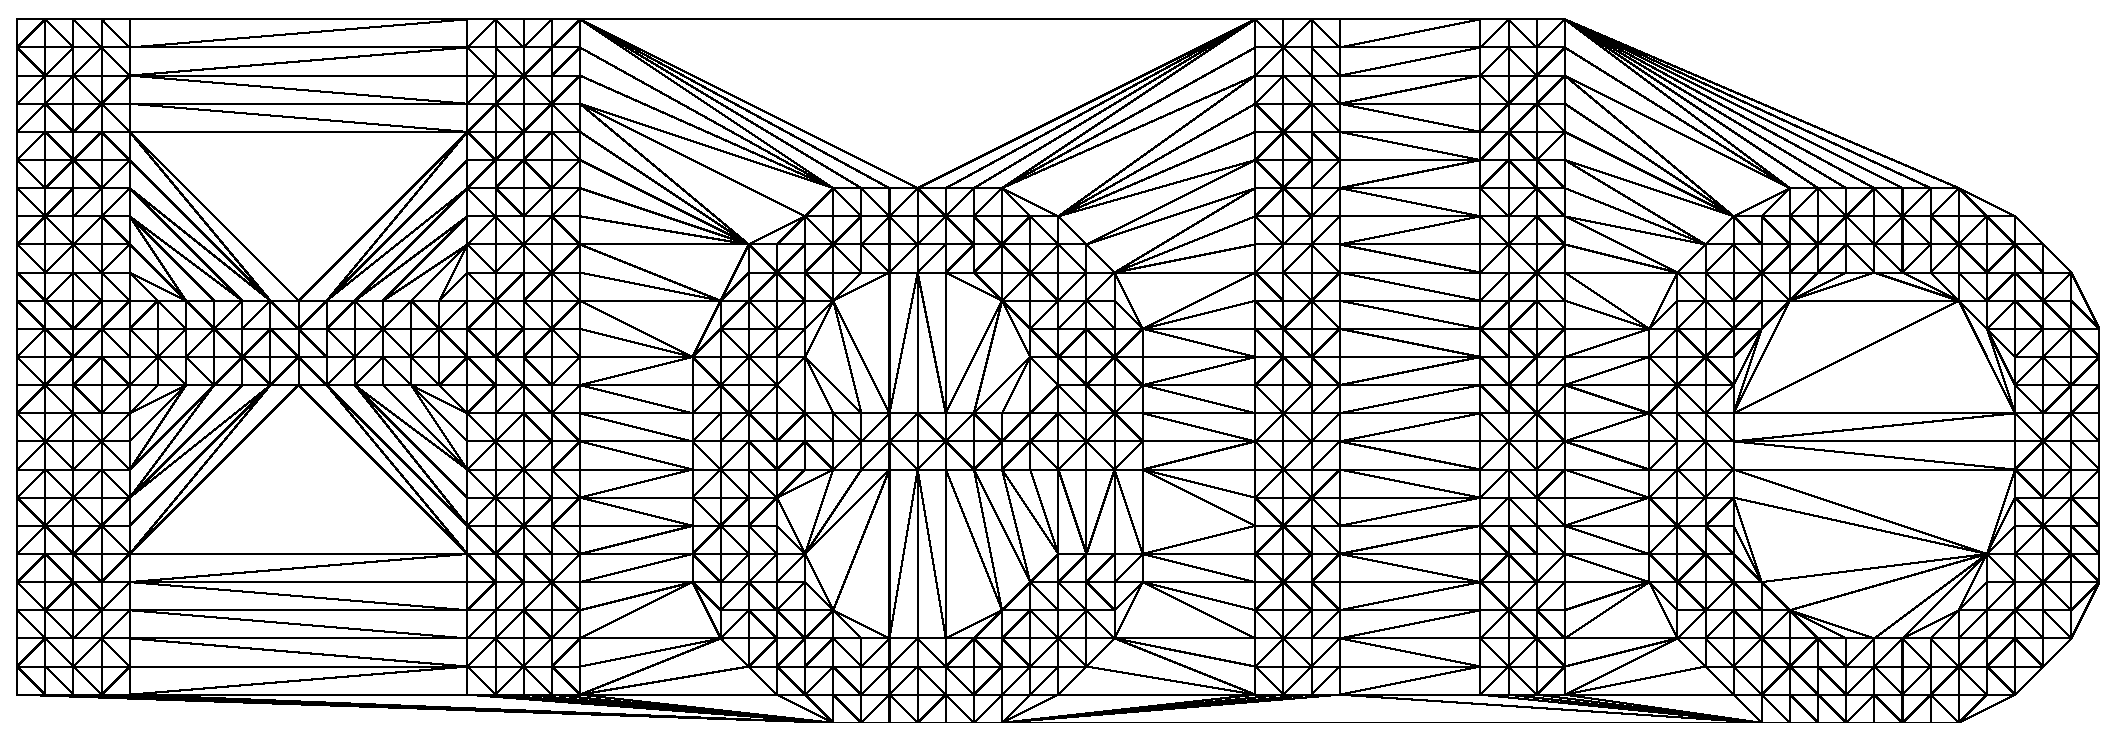
\includegraphics[width=0.8\textwidth]{helloTri}
  \caption{``Hello'' 点阵的 Delaunay 三角化网格}\label{fig:helloTri}
\end{figure}

我在 \cite{wiki:EMST} 上找到了更好的办法:先找到这 $n$ 个点的 Delaunay
三角化 (Delaunay Triangulation) 网格,然后找这个网格图上的 EMST 即是整
个完全图的 EMST。寻找 Delaunay 三角化网格的时间复杂度为 $O(n\log n)$,
生成的网格也只有 $O(n)$ 条边,所以最后整个算法的时间复杂度为 $O(n\log
n)$。

关于 Delaunay 三角化我用的是 \cite{Berg:2008:CGA:1370949} 里面描述的算
法,在实现过程中还发现那个算法有瑕疵,写信给作者指出,他也承认了。不过
他认为我给的修正也未必正确,却没有指出错在哪里,这我就不管了。之后最小
生成树用的还是 Kruskal 算法,并查集除了生成迷宫之外又被用到了一次。

\begin{figure}[htbp]
  \centering
  \begin{minipage}{0.5\textwidth}
    \centering
    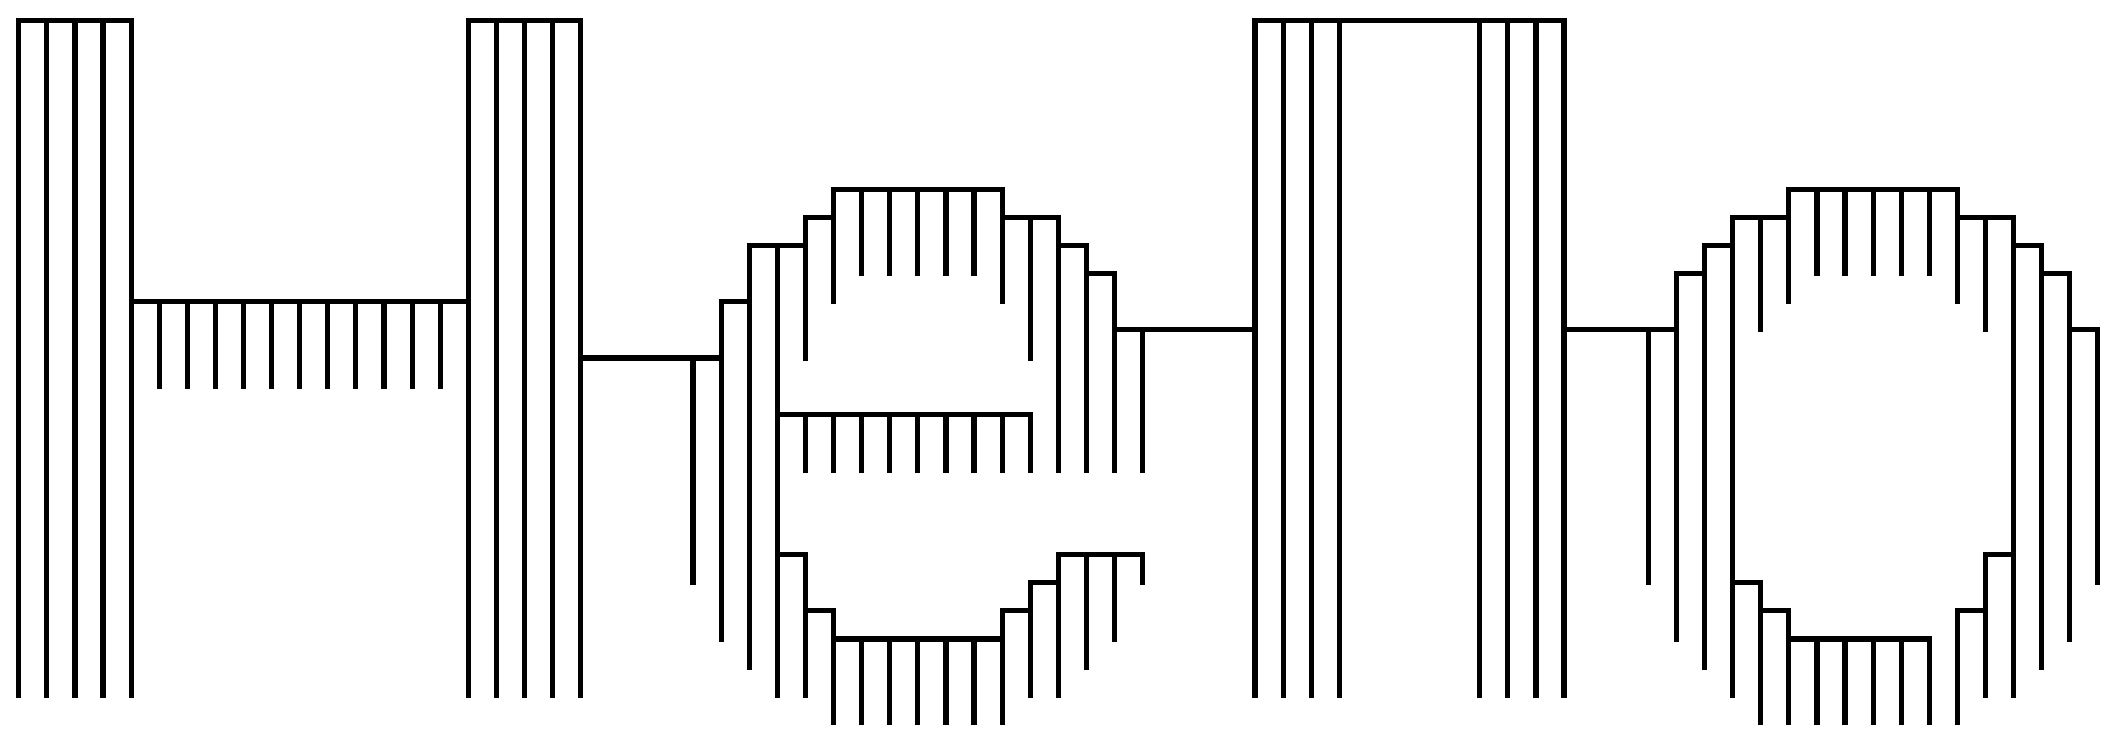
\includegraphics[width=0.95\linewidth]{helloEMST}
    \caption{``Hello'' 点阵的最小生成树}\label{fig:helloEMST}
  \end{minipage}%
  \begin{minipage}{0.5\textwidth}
    \centering
    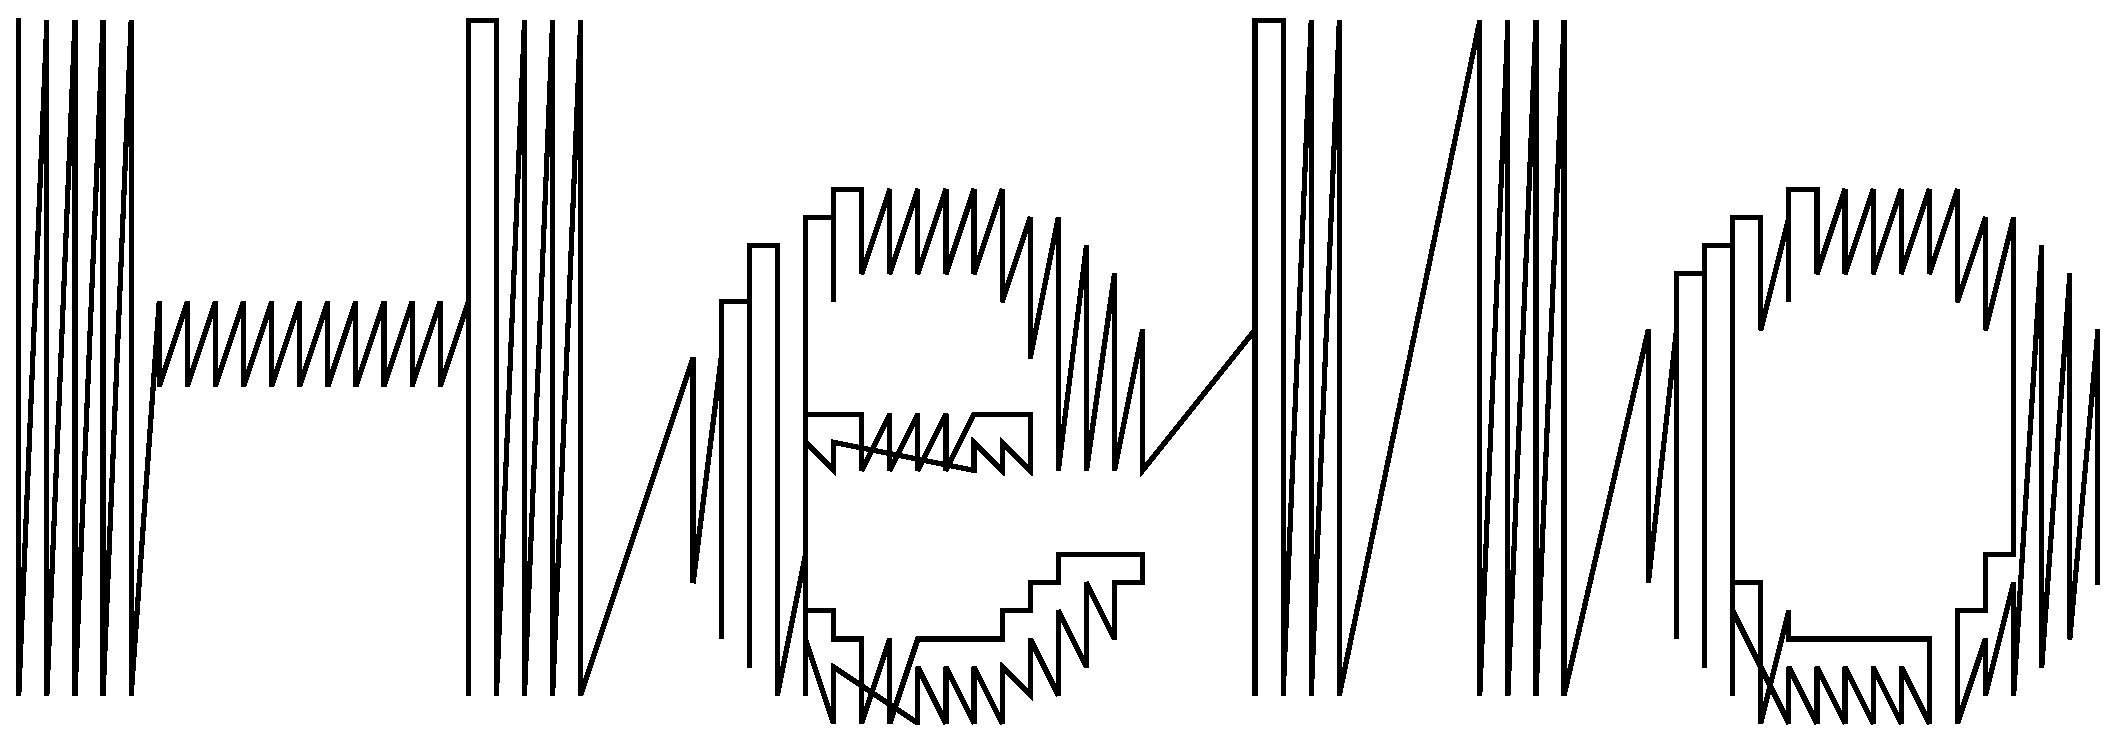
\includegraphics[width=0.95\linewidth]{helloInit}
    \caption{``Hello'' 点阵的初始路径}\label{fig:helloInit}
  \end{minipage}
\end{figure}

有了最小生成树,设其各条边长度之和为 $l$,这个 $l$ 也是 TSP 最优解的下
界。根据这棵树求一个初始的环路很简单,只要深度优先的遍历整棵树,把遍历
过程中经过的点作为“足迹”记下来。这个足迹包括回溯时经过的父结点,确保整
个足迹中相邻两个点总构成树上的一条边。得到这样的足迹之后,再遍历这个足
迹,按顺序将遇到的结点记录下来,遍历过程中跳过已经记录的结点。这样得到
的一条回路根据平面上三角形两边之和大于第三边的三角不等式,长度不会超过
$2l$。

用相同的思路,再做些修正,就能解决求指定了起点 $s$ 和终点 $t$ 的遍历路
径,要求长度也不超过 $2l$ 的问题。指定了起点 $s$ 之后,首先要把最小生成
树转化为以 $s$ 为根结点的树。转化后当然还是最小生成树,这只是数据结构上
的变化,不难做,画出来还是和原来一样的。以 $s$ 为根结点能保证遍历足迹得
到的路径以 $s$ 开头,却不能保证以 $t$ 结尾。这该如何解决呢?可以重新思
考一下所谓“足迹”到底是什么样子的,注意到足迹包括了回溯时经过的父结点,
这意味着对以 $a$ 为根结点的子树的足迹一定是以 $a$ 开头,也以 $a$ 结尾的。
整个足迹除了叶子结点之外,就是层层叠叠嵌套起来的结点对。只要不改变嵌套
的层次关系,同一级别的嵌套调换顺序不影响足迹的本质,这在直觉上也是好理
解的:我们并没有规定访问子结点的顺序。于是只要适当调换一下访问子结点的
顺序,让 $t$ 所在的各级别的子树都最后访问即可。这样形成的足迹按照原先的
处理办法遍历并记录新遇到的结点,当然,由于 $t$ 未必是叶子结点,所以遍历
前要对 $t$ 再做特别处理,只保留整个足迹中最后那个 $t$。这样我们就能得到
一个指定了起点和终点的初始路径,长度不超过 $2l$。

\subsubsection{Lin-Kernighan 算法}
现在初始的路径有了,下面就是逐步调整的过程了。根据三角不等式,四边形的
对角线长度之和大于任一对对边之和,这意味着经过同样点的不交叉路径一定比
交叉的路径要短。所以最简单的要做的就是调整所有交叉的路径,使其不再交叉。
用形式化的语言来说,对于一条路径 $(i_0,\dots,i_{n-1})$ 而言,若存在
$0< p < q < n-1$,使得
\begin{equation}
  |i_{p-1},i_p| + |i_q,i_{q+1}| > |i_{p-1},i_q| + |i_p,i_{q+1}|
\end{equation}
则路径可以被调整为
\begin{equation}\label{eq:pqOpt}
  (i_0,\dots,i_{p-1},i_q,i_{q-1},\dots,i_{p+1},i_p,i_{q+1},\dots,i_{n-1})
\end{equation}

这是用新的连接关系 $(i_{p-1},i_q)$ 和 $(i_p,i_{q+1})$ 替换了原有的连
接关系 $(i_{p-1},i_p)$ 和 $(i_q,i_{q+1})$。造成的效果则是把第 $p$ 个位
置到第 $q$ 个位置的路径翻转了一下。

如果不能替换一条路径的 $\lambda$ 处连接方式来使这条路径更短,则称这条路
径为 $\lambda$ 阶最优的。显然,一条路径没有交叉当且仅当它是 $2$ 阶最优
的。$n$ 个点的 TSP 路径当然要是 $n-1$ 阶最优的。所以一个自然的想法就是
继续逐步优化,使得路径变成 3 阶最优,4 阶最优乃至更高阶。但 Lin 和
Kernighan 通过实验证明 4 阶最优不见得比 3 阶最优好多少但算法却复杂太多
了。而他们俩提出的 Lin-Kernighan 算法则可以被认为是一种“可变 $\lambda$
阶的调优”。算法的核心是试图找到一个由翻转组成的序列,使得对原路径做了这
一系列可能很长的翻转操作之后,得到的新路径比较短。如果找到了,那么就做
这些翻转操作,然后继续新一轮的搜索。翻转过程中的中间路径可能比原路径更
长,但只要一个翻转序列的最终结果是个更短的路径就可以了。说它是一种“可变
$\lambda$ 阶的调优”则是因为改变 $\lambda$ 处连接方式总能通过一系列的翻
转操作来达到。

为了说得更清楚些,先做一些符号约定。所有平面上的点都用小写希腊字母表示。
函数 $d(\alpha,\beta)$ 表示点 $\alpha$ 和 $\beta$ 之间的欧氏距离;
$n(\alpha)$ 表示路径中紧随在 $\alpha$ 之后的那个点;$p(\alpha)$ 表示路
径中 $\alpha$ 前的那个点。根据这个符号约定,$2$ 阶优化就可以这么做了:
对于路径中任意一点 $\alpha$,若能找到另外一个点 $\beta$,使得
\begin{equation}\label{eq:2opt}
  d(\alpha,n(\alpha)) + d(\beta, n(\beta)) > d(\alpha, \beta) +
  d(n(\alpha), n(\beta))
\end{equation}
那么就可以通过翻转操作 $flip(n(\alpha), beta)$ 来得到一个更短的路径。缩短的长度是
\begin{equation}\label{eq:diff}
  d(\alpha,n(\alpha)) - d(n(\alpha), n(\beta)) + d(\beta, n(\beta)) -
  d(\alpha, \beta)
\end{equation}

Lin-Kernighan 算法扩展了上述想法,扩展有两方面:首先不再要求
(\ref{eq:2opt}) 这么强的条件,而只要求
\begin{equation}
  d(\alpha,n(\alpha)) - d(n(\alpha), n(\beta)) > 0
\end{equation}
因为条件放宽,所以 (\ref{eq:diff}) 的差值不再一定大于 0。故而第二个扩展
就是继续迭代,意思是并不是找到一个 $\beta$ 就停了,而是会继续找其它的符
合条件的 $\beta$,把历次的 (\ref{eq:diff}) 累加起来记为 $\Delta$。记下
迭代过程中使 $\Delta$ 最大且大于 0 的 $\beta$ 序列,然后依照序列顺序进
行 $flip(n(\alpha), \beta)$ 的翻转操作,就能得到最短的路径了。

整个 Lin-Kernighan 算法的核心思想就这么简单,要做的就是根据候选路径上各
点做上述搜索,若能找到用于改进的翻转序列则改进之。算法的核心就说到这里,
但离能据此实现还远得很。还有大量的细节尚未说明,比如如何寻找合适的
$\beta$,穷举是非常慢的;再比如如何高效的实现反转操作等等。这里限于篇幅
就不再详细介绍了,有兴趣的读者可以去看技术报告 \cite{1999finding}。在找
$\beta$ 的过程中,前面提到的 Delaunay 三角化网格也又一次发挥了作用。

\subsection{修正 TSP 路径为迷宫解路径}
用 Lin-Kernighan 可以得到 TSP 的一个近似解。近似解意味着它总长度已经很
小,但由于不是最优解,所以非但不能保证横平竖直,就连自身不交叉都未必能
保证。所以要将近似解变成我们需要的迷宫解路径,需要两种修正,一种是把交
叉变成非交叉,一种是把歪斜路径变成横平竖直。

把交叉路径变成非交叉并不难,只要找到交叉的线段后,翻转交叉线段之间的路
径解开交叉即可。考虑到 $n$ 个点的 TSP 近似解有 $O(n)$ 条线段,两两判断
是否交叉的时间复杂度是 $O(n^2)$,有点高。所以我在这步用的是计算几何中经
典的 Bentley-Ottmann 算法,它的时间复杂度是 $O(n\log n+k\log n)$,$k$
是交叉点数量,近似解中 $k=O(n)$。具体实现这个算法的难度不小,因为和教科
书上一般介绍的情况不同,处理实际应用时需要考虑所有诸如重合,多条线段交
于一点能边界状况,我参考了 \cite{Berg:2008:CGA:1370949} 中的处理办法。
我有时间会另外写文章详细阐述这里面的各种考量,这篇文章里就不细说了。

把歪斜路径变成横平竖直也不难,沿着近似解路径一路走过去,遇到斜线就尝试
能不能通过增加或减少附近的点来改走直线。若不成,则返回失败,对路径做随
机扰动后重新求解,再修正。这一算法需要判断某点在不在已有的路径上,若每
次都遍历查询效率太差,所以需要一个快速的办法判定点在不在路径上,且根据
需要往路径上增删点。定位快可以用二分查找在平衡二叉树上查,插删结点方便
可以用双向链表,两者都要则可以把两种数据结构结合在一起。平衡二叉树上每
个结点还有两个指针,指向前趋和后继。最后我是把红黑树及双向链表混合在一
起,来做修正路径的数据结构的。

\section{总结}
\GridMaze{} 根据点阵生成迷宫,使得迷宫的解能形成一开始点阵的形状。做这
个程序的动机虽然简单,但从动机到真正做出来就不是个简单的事情了。连点成
线和最有名的 NP 完全问题 TSP 有关,等得到解路径后,生成迷宫就相对容易些
了。iPad 版的程序从最早代码提交到最后提请发布,我花了 5 个月的业余时间,
里面有笑有泪,收获不小。这篇报告也算是对这番辛苦的一个交代吧。

\bibliographystyle{unsrt}
\bibliography{algorithm}
\end{document}
